
\documentclass[12pt, a4paper, oneside, romanian]{teza-upb}
\setcounter{secnumdepth}{3}
\setcounter{tocdepth}{3}
\usepackage{babel}
\usepackage{graphicx}
\usepackage{color}
\usepackage{float}

\usepackage[
  bookmarks,
  bookmarksopen=true,
  pdftitle={Chatbot medical},
  linktocpage]{hyperref}


\singlespacing

%%%%%%%%%%%%%%%%%%%%%%%%%%%%%%%%%%%%%%%%%%%%%%%%%%%%%%%%cod colorat
\usepackage{listings}
 
\definecolor{codegreen}{rgb}{0,0.6,0}
\definecolor{codegray}{rgb}{0.5,0.5,0.5}
\definecolor{codepurple}{rgb}{0.58,0,0.82}
\definecolor{backcolour}{rgb}{0.95,0.95,0.92}

\lstdefinestyle{mystyle}{
	language=Matlab,
 %   backgroundcolor=\color{backcolour},   
    commentstyle=\color{codegreen},
    keywordstyle=\color{blue},
    numberstyle=\tiny\color{codegray},
    stringstyle=\color{codepurple},
	basicstyle=\ttfamily\scriptsize,
    breakatwhitespace=false,         
    breaklines=true,                 
    captionpos=b,                    
    keepspaces=true,                 
    numbers=left,                    
    numbersep=5pt,                  
    showspaces=false,                
    showstringspaces=false,
    showtabs=false,                  
    tabsize=2
}
 
\lstset{style=mystyle}
%%%%%%%%%%%%%%%%%%%%%%%%%%%%%%%%%%%%%%%%%%%%%%%

\begin{document}

\author{Miron Marta-Florentina}

\title{Chatbot medical}


\facultatea{Facultatea de Electronică, Telecomunicații și Tehnologia Informației}
\tiplucrare{licență}
%\tiplucrare{dizertație}
\domeniu{Electronică, Telecomunicații și Tehnologia Informației}
\catedra{Telecomunicații}
\campus{Leu} 
\program{Electronică Aplicată}
\titlulobtinut{Inginer}
%\titlulobtinut{Master}
\director{Prof. Dr. Ing. Bogdan-Emanuel Ionescu} 

\submissionmonth{Iunie} 
\submissionyear{2026} 

\beforepreface
\listoffigures
\listoftables
\abbreviations{ 
  RNN = Rețea Neuronală Recurentă\\
  LLM = Large Language Model\\
  RAG = Retrieval-Augmented Generation\\
  NLP = Natural Language Processing\\
  API = Application Programming Interface
  
}
%\preface{}
\afterpreface 

\chapter*{Introducere}
\section{Motivația alegerii temei}

Interesul meu pentru inteligența artificiala a apărut încă din timpul liceului, când, în cadrul orelor de Informatică, au fost discutate pentru prima dată schimbările pe care aceste tehnologii le-ar putea produce în societate și pe piața muncii. La acel moment, subiectul părea mai degrabă unul teoretic si cu putin impact in viitorul apropiat. Cu toate acestea, pe măsură ce tehnologia a evoluat, ideile despre sisteme capabile să depășească performanțele umane în anumite domenii, precum jocul de șah sau analiza datelor, au început să devină realitate.

În prezent, evoluția rapidă a inteligenței artificiale confirmă faptul că aceste transformări nu mai aparțin unui viitor îndepărtat, ci fac deja parte din realitatea cotidiană. Tocmai această dezvoltare accelerată a reprezentat una dintre principalele motivații pentru alegerea temei detaliate în rândurile următoare. Interesul pentru înțelegerea modelelor moderne de inteligență artificială și dorința de a folosi aceste tehnologii la îmbunătățirea procesului de învățare din surse responsabile și sigure au condus spre ideea dezvoltării unui chatbot.

Alegerea domeniului medical reprezintă un caz particular de aplicabilitate a soluției propuse, aceasta fiind concepută scalabil, încât să poată fi adaptată și extinsă cu ușurință pentru prelucrarea și folosirea altor tipuri de documente. În plus, domeniul medical este unul sensibil în ceea ce privește utilizarea inteligenței artificiale ca suport pentru informare și documentare, motiv pentru care proiectarea unui astfel de sistem necesită o abordare orientată către limitarea riscului de furnizare a unor informații eronate sau verificate insuficient.

Această temă îmbină două direcții de interes majore: pe de o parte, studiul sistemelor conversaționale și al procesării limbajului natural, iar pe de altă parte, aplicarea acestora într-un domeniu de interes real, în care accesul rapid la informație poate sprijini procesul de învățare, documentare și verificare pentru studenți, cadre didactice și profesioniști din domeniul medical.


\section{Scopul și obiectivele lucrării}

Această lucrare își propune proiectarea și implementarea unui chatbot medical bazat pe modele lingvistice de mari dimensiuni, asistat de mecanisme de regăsire a informației relevante din surse validate.

Obiectivele principale ale lucrării sunt:
\begin{itemize}
    \item analizarea fundamentelor teoretice necesare: rețele neuronale, arhitectura Transformer, LLM și RAG;
    \item proiectarea unei arhitecturi agentice capabile să decidă când este necesară regăsirea de context și cum este construit promptul final;
    \item implementarea unui flux robust de răspuns, care include validarea automată a rezultatului și mecanisme de reluare (\textit{retry});
    \item evaluarea comparativă a mai multor modele LLM și furnizori, în funcție de calitatea răspunsului și stabilitate;
    \item evidențierea limitărilor actuale și formularea unor direcții de extindere pentru utilizare practică în domeniul medical.
\end{itemize}

\section{Sumarul lucrării}

Teza este structurată în 4 capitole principale:
\begin{itemize}
    \item Capitolul 1 (Fundamente teoretice) prezintă conceptele de bază necesare înțelegerii lucrării, incluzând arhitectura Transformer, modelele lingvistice de mari dimensiuni și mecanismele de tip Retrieval-Augmented Generation, dar și modelele ce stau la baza Inteligenței Artificiale.
    \item Capitolul 2 cuprinde prezentarea detaliată a tehnologiilor folosite în proiect.
    \item Capitolul 3 descrie arhitectura proiectului și împărțirea în agenți.
    \item Capitolul 4 conține prezentarea rezultatelor și comparația acestora în funcție de modelul LLM folosit.
\end{itemize}


\cleardoublepage
\chapter{Fundamente teoretice}

\section{Rețele neuronale artificiale}
    \subsection{Structura unei rețele neuronale}

Învățarea profundă se bazează pe construirea unor niveluri succesive de reprezentare a datelor, fiecare nivel extrăgând caracteristici tot mai abstracte din informația de intrare. Aceste reprezentări sunt organizate în straturi și sunt învățate prin intermediul rețelelor neuronale artificiale, o clasă de modele utilizate pentru identificarea relațiilor complexe și neliniare din date.

O rețea neuronală artificială poate fi privită ca un aproximator de funcții, fiind alcătuită dintr-un strat de intrare, unul sau mai multe straturi ascunse și un strat de ieșire. Fiecare strat este format din unități de calcul numite neuroni artificiali, conectați între ei prin intermediul unor ponderi.

Fiecare neuron calculează o combinație liniară a valorilor de intrare, realizată prin înmulțirea acestora cu ponderile asociate conexiunilor. Rezultatul obținut este transmis unei funcții de activare, care introduce neliniaritate în model și determină ieșirea neuronului. În primul strat ascuns, datele provin direct din stratul de intrare, iar în straturile următoare informația este transmisă de la stratul precedent. \cite{curs_IA}

\begin{figure}[h]
    \centering
    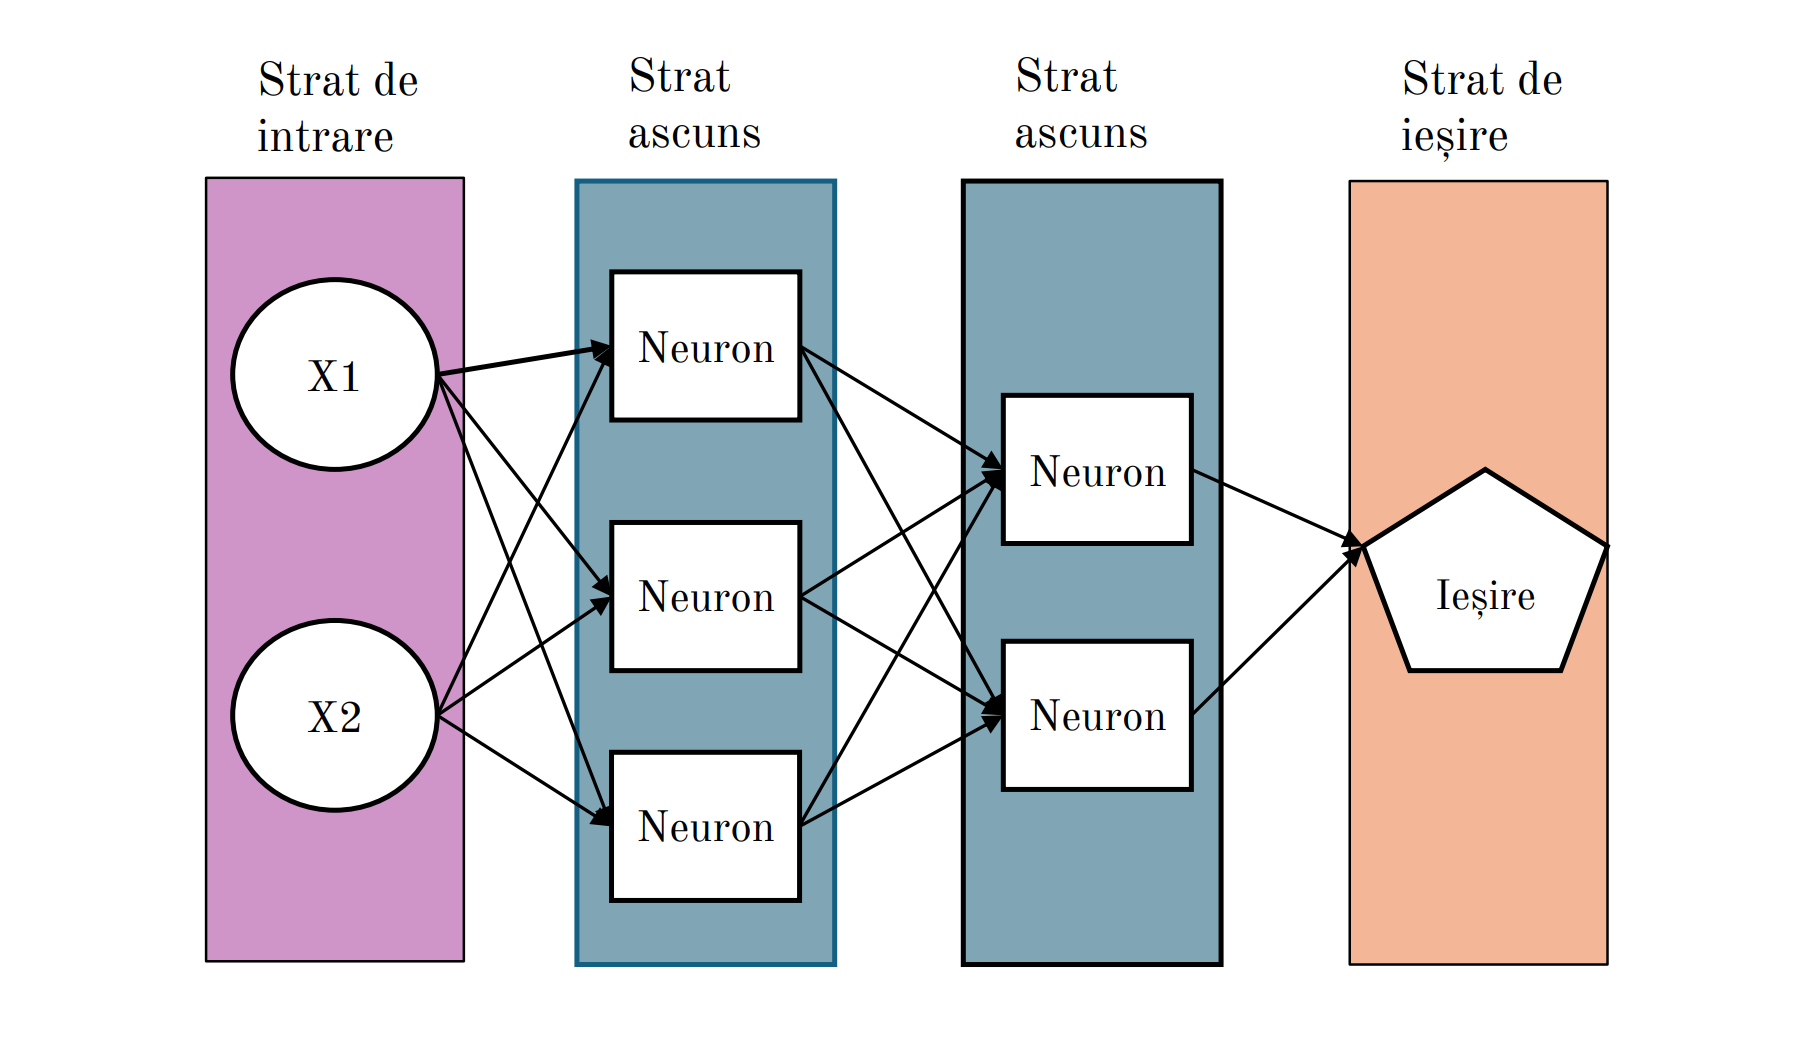
\includegraphics[width=0.9\textwidth]{figuri/retea_neuronala.png}
    \caption{Arhitectura unei rețele neuronale \cite{curs_IA}}
    \label{fig:retea-neuronala}
\end{figure}


    \subsection{Algoritmul de antrenare: Gradient Descent și Backpropagation}

    
Ponderile inițiale ale modelului nu sunt, în general, optime, motiv pentru care se utilizează tehnici de antrenare pentru ajustarea acestora în funcție de setul de date de antrenare.


Scopul unui algoritm de învățare automată este reducerea erorii de generalizare
a modelului. Această eroare reprezintă diferența dintre predicțiile modelului și
valorile reale ale datelor provenite din distribuția reală a fenomenului analizat
și este cunoscută în literatură sub denumirea de risc.

În mod ideal, antrenarea unui model ar presupune minimizarea erorii de predicție pe întreaga distribuție reală a datelor. În practică însă, această distribuție nu este cunoscută, iar modelul are acces doar la un set finit de exemple de antrenare. Din acest motiv, optimizarea modelului se realizează prin minimizarea erorii medii calculate pe setul de date disponibil, proces cunoscut sub denumirea de minimizarea riscului empiric.

Astfel, în locul riscului real se minimizează riscul empiric, care reprezintă
media erorilor calculate pentru exemplele din setul de antrenare. Procesul de
antrenare bazat pe această idee este cunoscut sub denumirea de \textit{empirical
risk minimization}.

Deși această abordare permite formularea problemei de învățare ca o problemă
de optimizare, ea poate conduce la fenomenul de supraînvățare
(\textit{overfitting}), în special în cazul modelelor cu capacitate mare.
În astfel de situații, modelul poate învăța foarte bine datele de antrenare,
dar performanța sa pe date noi poate fi redusă.

În practica modernă a învățării profunde, optimizarea modelelor se realizează
de obicei prin metode bazate pe algoritmul \textit{gradient descent}, care
permite actualizarea iterativă a parametrilor modelului în direcția reducerii
funcției de pierdere \cite{goodfellow2016}.

Calculul gradientului necesar pentru actualizarea parametrilor unei rețele
neuronale este realizat prin algoritmul \textit{backpropagation}. Acest algoritm
ajustează în mod iterativ ponderile conexiunilor din rețea astfel încât
diferența dintre ieșirea produsă de model și valoarea dorită să fie cât mai mică.
Procesul presupune propagarea erorii de la stratul de ieșire către straturile
anterioare ale rețelei, determinând contribuția fiecărui parametru la eroarea
totală. În urma acestor actualizări, neuronii din straturile ascunse ajung să
reprezinte caracteristici relevante ale datelor, ceea ce permite modelului să
învețe relațiile existente în setul de antrenare \cite{rumelhart1986learning}.


\section{Rețele neuronale recurente (RNN)}
    \subsection{Arhitectura RNN}

Rețelele neuronale recurente (RNN) se numără printre primele arhitecturi dezvoltate pentru procesarea datelor secvențiale, fiind utilizate în aplicații precum modelarea limbajului sau traducerea automată. Un element esențial al acestor rețele este capacitatea de a păstra o stare internă (hidden state), care stochează informații despre intrările anterioare din secvență. Prin intermediul acesteia, RNN-urile pot stoca și modela dependențele temporale existente între elementele secvenței. \cite{dataversity} 

\begin{figure}[H]
\centering

\includegraphics[width=0.9\textwidth]{figuri/RNN.png}
\caption{Arhitectura unei rețele neuronale recurente \cite{jurafsky2023}}
\label{fig:rnn}
\end{figure}

Starea internă a rețelei este actualizată la fiecare pas temporal în funcție de
intrarea curentă și de valoarea stării ascunse din pasul anterior. În acest mod,
ieșirea modelului nu depinde doar de datele curente, ci și de informațiile
procesate anterior. Astfel, rețeaua poate păstra un anumit context al secvenței,
care influențează predicțiile realizate la pașii următori.

Deși introducerea acestei dimensiuni temporale $h_t$ poate face arhitectura să pară
mai complexă decât rețelele neuronale clasice de tip feedforward, mecanismul
de calcul rămâne similar. La fiecare pas temporal, modelul primește vectorul
de intrare și starea ascunsă din momentul precedent, iar pe baza acestora
calculează noua stare internă a rețelei. Conexiunile recurente dintre stările
ascunse permit modelului să utilizeze informațiile din trecut pentru a produce
ieșirea corespunzătoare intrării curente \cite{jurafsky2023}.

\begin{figure}[h]
    \centering
    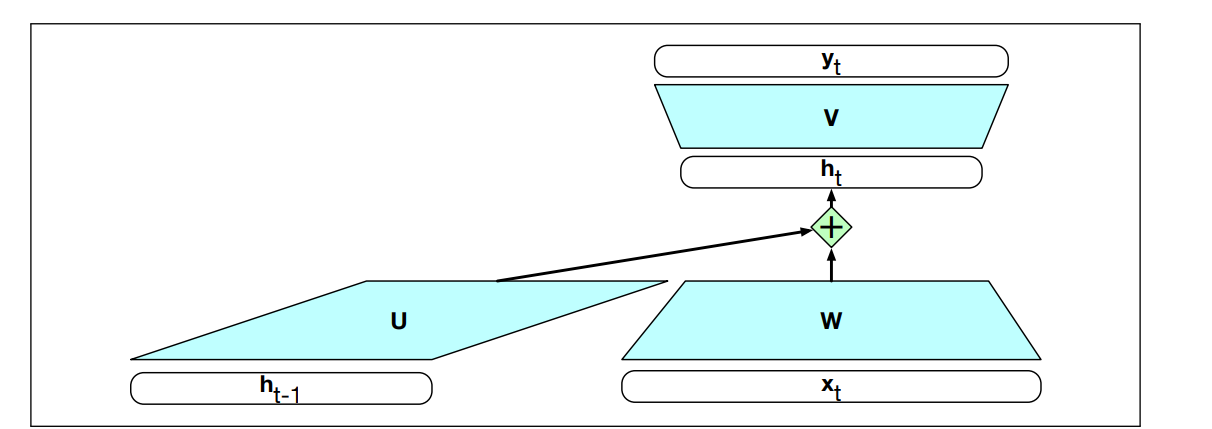
\includegraphics[width=0.9\textwidth]{figuri/RNN_desfasurat.png}
    \caption{Arhitectura RNN desfășurată \cite{jurafsky2023}}
    \label{fig:rnn-desfasurat}
\end{figure}


    \subsection{Limitări ale RNN}

Antrenarea rețelelor neuronale recurente poate fi dificilă
în cazul aplicațiilor care necesită utilizarea unor informații aflate la
o distanță mare în cadrul secvenței. Deși, teoretic, RNN-urile au acces
la întreaga secvență anterioară, informația codificată în stările ascunse
tinde să fie mai degrabă locală, fiind mai relevantă pentru cele mai
recente elemente ale secvenței și pentru deciziile luate recent.

În mod ideal, o rețea ar trebui să fie capabilă să păstreze informații
aflate la distanță în secvență până în momentul în care acestea devin
relevante, procesând în același timp corect elementele intermediare.
În practică însă, straturile ascunse și ponderile asociate acestora sunt
nevoite să îndeplinească simultan două roluri: să furnizeze informații
utile pentru decizia curentă și, în același timp, să actualizeze și să
transmită mai departe informațiile necesare pentru deciziile viitoare.

O altă dificultate apare în timpul procesului de antrenare, atunci când eroarea trebuie propagată înapoi prin mai mulți pași temporali.
În această situație, gradientul funcției cost este supus unor multiplicări
repetate, determinate de lungimea secvenței. Ca urmare, valorile
gradientului pot scădea progresiv până aproape de zero, fenomen
cunoscut sub denumirea de \textit{vanishing gradient}. 
        \subsubsection{Problema vanishing gradient}

Această problemă apare în special în cazul rețelelor neuronale recurente, unde procesul de antrenare implică propagarea erorii prin mai mulți pași temporali. În timpul
\textit{backpropagation through time}, gradientul este multiplicat
în mod repetat cu aceleași ponderi ale rețelei. Dacă valorile acestor
ponderi sunt mici, gradientul poate scădea rapid spre zero,
ceea ce face dificilă actualizarea eficientă a parametrilor
rețelei pentru informații aflate la distanță în secvență. \cite{jurafsky2023}
    \subsection{Modele îmbunătățite: LSTM și GRU}

Pentru a depăși limitările rețelelor neuronale recurente clasice, au fost
propuse arhitecturi mai complexe, dintre care cea mai utilizată este
\textit{Long Short-Term Memory} (LSTM), introdusă de Hochreiter și
Schmidhuber în 1997 \cite{hochreiter1997long}. Rețelele LSTM abordează
problema gestionării contextului prin separarea a două procese
esențiale: eliminarea informațiilor care nu mai sunt relevante și
păstrarea informațiilor utile pentru deciziile ulterioare. Spre
deosebire de arhitecturile RNN clasice, în care modul de gestionare a
contextului este implicit, LSTM permite rețelei să învețe automat cum
să controleze fluxul informației de-a lungul secvenței.

Pentru a realiza acest lucru, LSTM utilizează unități neuronale
specializate care includ mecanisme de tip \textit{gates} (porți),
responsabile pentru controlul fluxului de informație care intră și
iese din celula de memorie.

Porțile (\textit{gates}) dintr-o rețea LSTM au rolul de a controla
fluxul de informație în cadrul celulei de memorie. Fiecare poartă
utilizează un strat de tip \textit{feedforward} urmat de o funcție de
activare sigmoid, care produce valori cuprinse între 0 și 1. Aceste
valori determină în ce măsură informația este transmisă mai departe
sau eliminată, permițând rețelei să păstreze doar informațiile
relevante pentru procesarea ulterioară.

\begin{figure}[h]
    \centering
    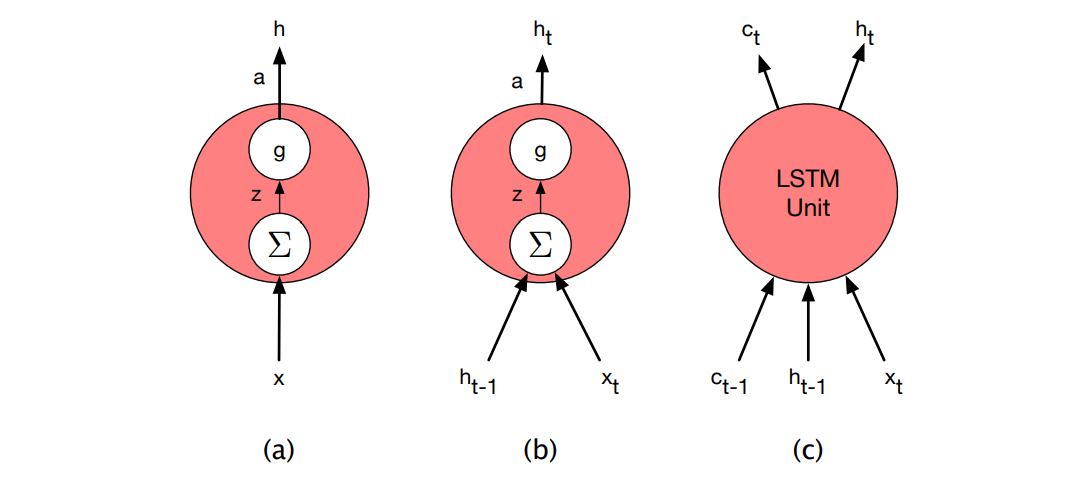
\includegraphics[width=0.9\textwidth]{figuri/Comparatie structura.png}
\caption{Arhitectura neuronului utilizat în rețele feedforward,
Rețele Neuronale Recurente (RNN) și rețele Long Short-Term Memory (LSTM) \cite{jurafsky2023}}
    \label{fig:comparatie-rnn-lstm}
\end{figure}

\section{Arhitectura Transformer}

Termenul Transformer a fost introdus pentru prima dată în articolul „Attention Is All You Need” \cite{vaswani2017attention} publicat în 2017 de către Vaswani și colaboratorii săi, în care autorii propun un model bazat exclusiv pe mecanismul de self-attention pentru procesarea secvențelor, fără utilizarea
recurenței specifice rețelelor neuronale recurente. Spre deosebire de arhitecturile bazate pe rețele neuronale recurente,
care procesează datele în mod secvențial, modelul Transformer permite
analizarea simultană a tuturor elementelor unei secvențe. Această
abordare facilitează paralelizarea calculelor și permite capturarea
dependențelor dintre elemente aflate la distanță în secvență.

    \subsection{Structura encoder–decoder}

La baza Transformerelor stă o arhitectură de tip encoder-decoder. Acest tip de arhitectură este utilizat pentru a transforma o secvență de intrare într-o secvență de ieșire, fiind frecvent întâlnită în aplicații precum traducerea automată \cite{sutskever2014sequence}.


Modelul este alcătuit din două componente principale. Encoderul primește secvența de intrare și o procesează element cu element, construind treptat o reprezentare internă a acesteia. La finalul procesării, informația este sintetizată într-un vector de context, care conține informația esențială despre întreaga secvență de intrare.

Acest vector de context este transmis către decoder, care generează secvența de ieșire pas cu pas. La fiecare pas, decoderul utilizează atât informația din vectorul de context, cât și elementele generate anterior, pentru a produce următorul element din secvență.
Un avantaj important al acestei arhitecturi este flexibilitatea în ceea ce privește lungimea secvențelor: numărul de elemente din intrare poate fi diferit de cel din ieșire. Encoderul și decoderul sunt antrenate împreună, astfel încât modelul să învețe relația dintre secvențele de intrare și cele de ieșire \cite{goodfellow2016}.

Totuși, în variantele clasice bazate pe rețele neuronale recurente, întreaga informație a secvenței de intrare este comprimată într-un singur vector de context. Această limitare poate duce la pierderi de informație, în special în cazul secvențelor lungi, deoarece modelul nu poate păstra eficient toate detaliile relevante.

Pentru a rezolva această problemă, au fost introduse ulterior mecanisme de tip attention, care permit modelului să acceseze direct diferite părți ale secvenței de intrare în timpul generării rezultatului \cite{bahdanau2015neural}.
\begin{figure}[H]
    \centering
    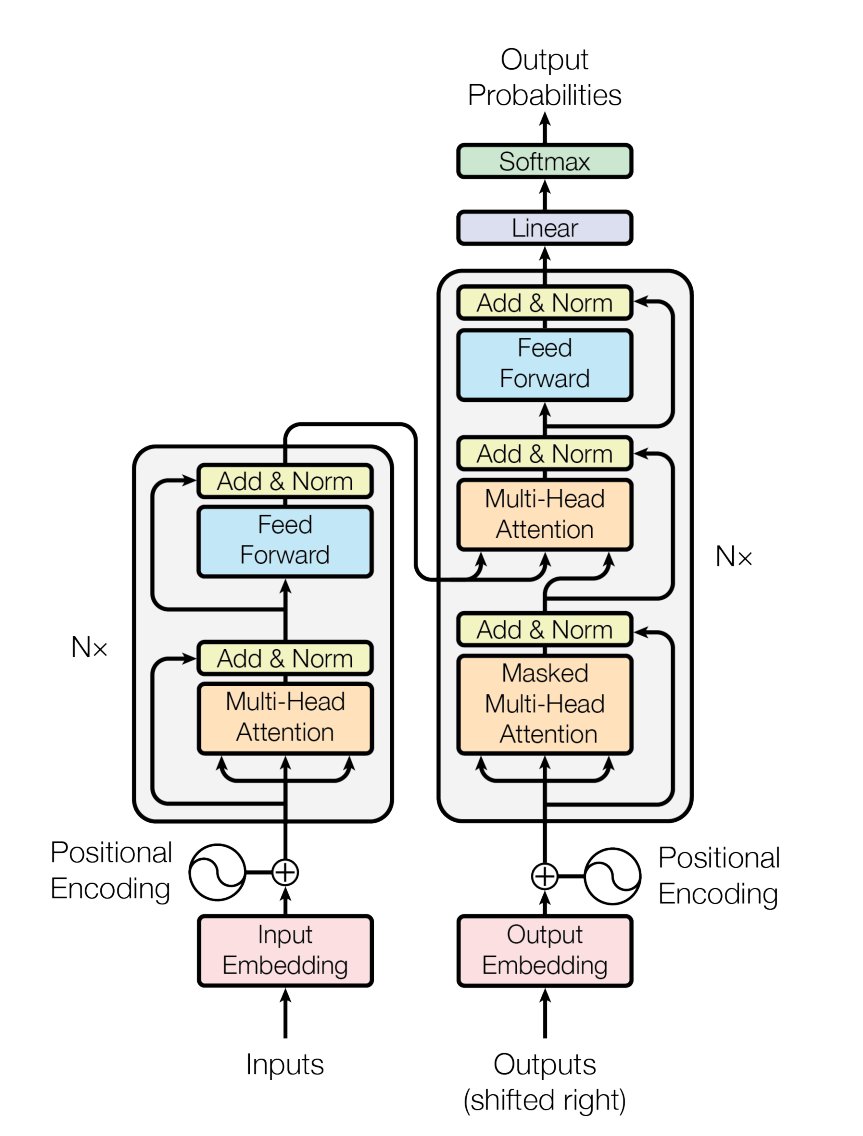
\includegraphics[width=0.8\textwidth]{figuri/encoder_decoder_ai.png}
    \caption{Arhitectura encoder-decoder \cite{vaswani2017attention}}
\end{figure}

    \subsection{Mecanismul self-attention}
    
Mecanismul de \textit{attention} poate fi privit ca un mod prin care
modelul decide asupra căror elemente din secvență trebuie să se
concentreze. Acesta primește o interogare (\textit{query}) și un set
de perechi cheie–valoare (\textit{key–value}), iar rezultatul este
obținut prin combinarea valorilor în funcție de cât de relevante sunt
pentru interogarea respectivă. Gradul de relevanță este determinat
prin compararea interogării cu fiecare cheie din secvență. 

Scorul de relevanță dintre query și fiecare key este calculat printr-o funcție de similaritate, de obicei produs scalar (dot-product), urmat de o normalizare cu funcția softmax.

Prin acest mecanism, modelul nu mai este limitat la un singur vector de context, ci poate accesa direct informații din întreaga secvență de intrare, ceea ce permite captarea mai eficientă a dependențelor pe termen lung \cite{vaswani2017attention}.
    
\section{Modele bazate pe Transformer}

Modelele Transformer reprezintă un tip de rețele neuronale capabile să înțeleagă contextul datelor secvențiale și să genereze informații noi pe baza acestora. Mai concret, un Transformer este un model de inteligență artificială care învață să interpreteze și să genereze text asemănător limbajului uman prin identificarea tiparelor din volume mari de date textuale. În prezent, transformerele sunt considerate unele dintre cele mai performante modele utilizate în procesarea limbajului natural (NLP) și pot fi privite ca o evoluție a arhitecturii encoder-decoder. Totuși, spre deosebire de arhitectura clasică encoder-decoder, care se bazează în principal pe rețele neuronale recurente (RNN) pentru a procesa informația secvențială, transformerele nu utilizează recurența. În schimb, aceste modele sunt proiectate pentru a înțelege contextul și semnificația datelor prin analizarea relațiilor dintre elementele unei secvențe. \cite{datacamp}

    \subsection{Modele lingvistice de mari dimensiuni (LLM)}

Modelele lingvistice de mari dimensiuni (LLM) sunt modele bazate pe arhitectura Transformer, antrenate pe volume foarte mari de date textuale, capabile să genereze text coerent și să rezolve diverse sarcini de procesare a limbajului natural \cite{brown2020language}.

Modelele lingvistice de mari dimensiuni (LLM) reprezintă o categorie de modele de limbaj bazate pe rețele neuronale cu un număr foarte mare de parametri, antrenate pe volume extinse de date textuale neetichetate, utilizând tehnici de învățare auto-supervizată. Prin procesul de pre-antrenare pe corpusuri de mari dimensiuni, aceste modele dobândesc capacitatea de a identifica tipare complexe, nuanțe semantice și relații contextuale în cadrul limbajului natural.

Datorită acestor proprietăți, modelele LLM pot fi utilizate într-o varietate de sarcini specifice procesării limbajului natural, precum generarea de text, traducerea automată, sumarizarea documentelor, răspunsul la întrebări sau analiza sentimentelor. De asemenea, adaptarea acestor modele pentru sarcini specifice, prin tehnici de fine-tuning, a condus la obținerea unor performanțe de ultimă generație în numeroase aplicații. 

\begin{figure}[H]
    \centering
    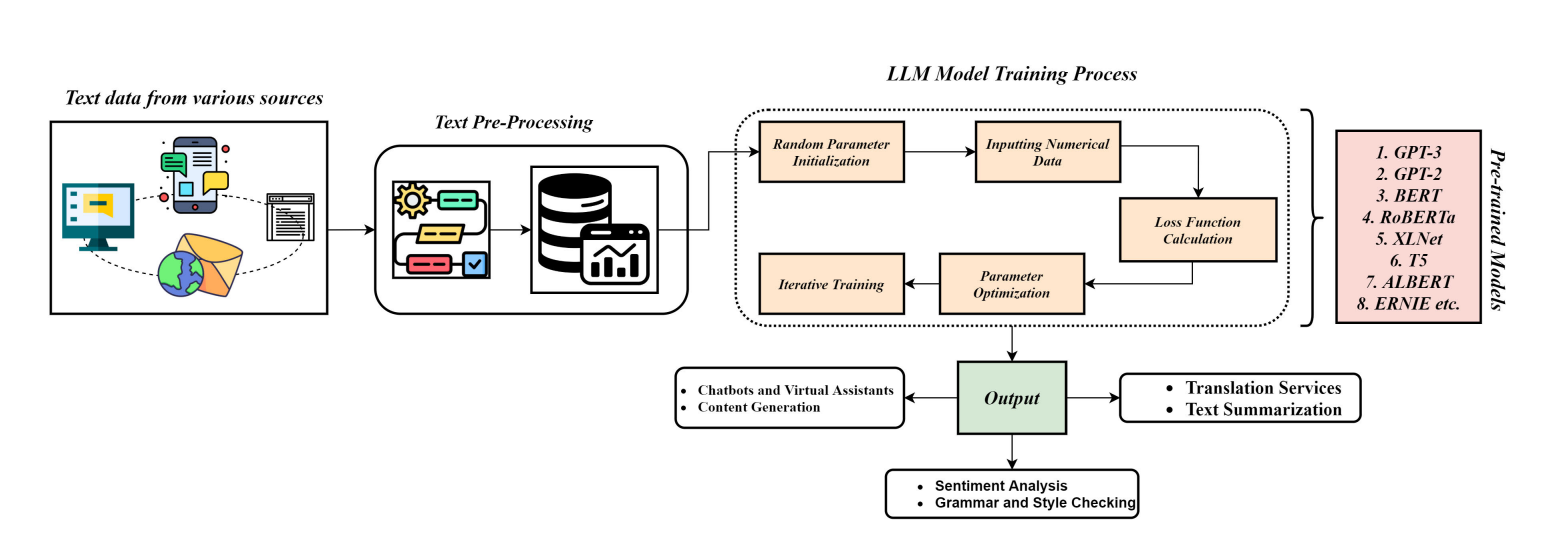
\includegraphics[width=\textwidth]{figuri/antrenare_llm.png}
    \caption{Procesul de antrenare al modelelor LLM \cite{llm_review_2024}}
    
\end{figure}

Arhitectura modelelor lingvistice de mari dimensiuni (LLM) presupune preluarea datelor text din multiple surse, urmată de transmiterea acestora către etapele de preprocesare. Procesul de antrenare include mai multe etape, precum inițializarea aleatorie a parametrilor, transformarea datelor în format numeric, calculul funcției de pierdere, optimizarea parametrilor și antrenarea iterativă a modelului.

După finalizarea antrenării, aceste modele pot fi utilizate pentru diverse sarcini de procesare a limbajului natural.

Odată cu dezvoltarea unor modele avansate, precum GPT, LLaMA sau Bard, și explorarea capacităților acestora în diverse aplicații, LLM-urile au devenit un domeniu esențial și extrem de activ în cercetarea actuală. În acest context, evaluarea performanței și a fiabilității acestor modele reprezintă o direcție importantă de studiu. \cite{llm_review_2024}.


    \subsection{Procesul de antrenare al modelelor LLM}
După cum se observă în figura 1.7, antrenarea LLM se poate împărți în mai mulți pași. După filtrarea datelor, 
tokenizarea reprezintă una dintre etapele esențiale de preprocesare în cadrul modelelor lingvistice de mari dimensiuni. Aceasta constă în împărțirea textului în unități discrete, denumite tokeni, care pot fi caractere, subcuvinte, simboluri sau cuvinte, în funcție de tipul modelului utilizat. În practică, sunt folosiți diverși algoritmi de tokenizare, precum WordPiece, UnigramLM sau Byte Pair Encoding (BPE), fiecare având o metodă specifică de segmentare a textului de intrare.

\begin{figure}[H]
    \centering
    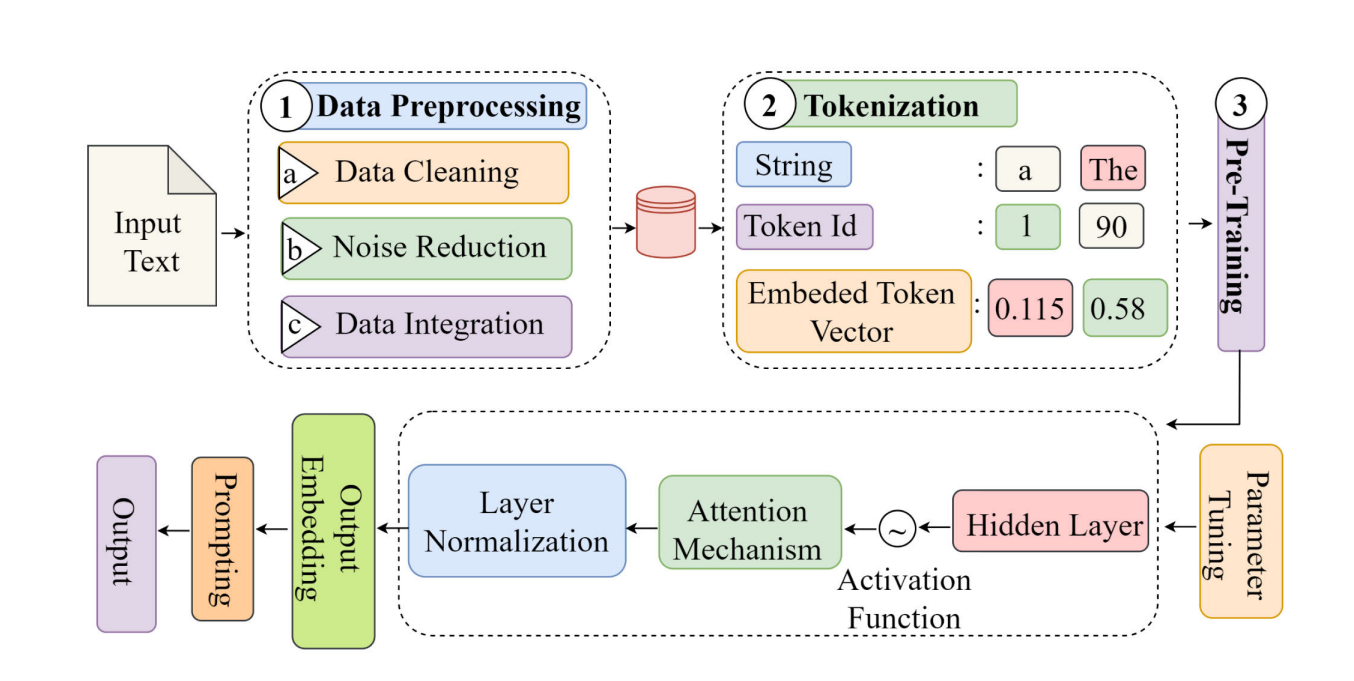
\includegraphics[width=0.8\textwidth]{figuri/LLM_stages.png}
    \caption{Pipeline complet LLM \cite{llm_review_2024}}
    
\end{figure}

După etapa de preprocesare, datele sunt transformate într-o formă numerică și utilizate în procesul de antrenare al modelului. Acesta include inițializarea parametrilor, calculul funcției de pierdere, optimizarea parametrilor și antrenarea iterativă, până la convergența modelului. Prin acest proces, modelul învață să identifice tipare și relații complexe în limbajul natural.

\section{Retrieval-Augmented Generation (RAG)}

Modelele lingvistice de mari dimensiuni pre-antrenate au demonstrat capacitatea de a stoca cunoștințe factuale în parametrii lor și de a obține performanțe ridicate atunci când sunt adaptate (fine-tuned) pentru sarcini specifice de procesare a limbajului natural. Cu toate acestea, capacitatea lor de a accesa și de a utiliza în mod precis aceste cunoștințe este limitată, ceea ce conduce la performanțe inferioare în cazul sarcinilor care necesită informații detaliate și actualizate.

De asemenea, dificultatea de a furniza surse clare pentru informațiile generate, precum și de a actualiza cunoștințele interne ale modelului, reprezintă provocări importante în utilizarea acestor modele. În acest context, au fost propuse abordări care integrează mecanisme de acces la surse externe de informație, prin utilizarea unei memorii non-parametrice.



\subsection{Conceptul de Retrieval-Augmented Generation}

O astfel de abordare este reprezentată de modelele de tip Retrieval-Augmented Generation (RAG), care combină memoria parametrică a modelului, învățată în timpul antrenării, cu o memorie externă, bazată pe regăsirea documentelor relevante. Această combinație permite îmbunătățirea procesului de generare a răspunsurilor, în special în sarcinile care necesită acces la informații suplimentare.

În această paradigmă, modelul nu se bazează exclusiv pe cunoștințele stocate în parametrii săi, ci utilizează un mecanism de regăsire pentru a identifica informații relevante dintr-o bază de date. Documentele recuperate sunt apoi utilizate ca sursă suplimentară de context în procesul de generare a răspunsului.

Această abordare contribuie la îmbunătățirea performanței în sarcini care necesită acces la cunoștințe detaliate sau actualizate și reduce riscul de generare a unor informații eronate, fenomen cunoscut sub denumirea de halucinații. În plus, RAG permite separarea cunoștințelor de model de datele utilizate, facilitând actualizarea informațiilor fără a fi necesară reantrenarea completă a modelului.

Prin integrarea mecanismelor de regăsire și generare, modelele RAG oferă un cadru flexibil pentru rezolvarea sarcinilor de procesare a limbajului natural, în special în aplicații care necesită acces la baze de cunoștințe extinse \cite{lewis2020retrieval} sau la proceduri interne.


\subsection{Arhitectura Retrieval-Augmented Generation}

Arhitectura modelelor de tip Retrieval-Augmented Generation este construită în jurul interacțiunii dintre două componente principale: un mecanism de regăsire a documentelor și un model de generare, integrate într-un cadru probabilistic unificat \cite{lewis2020retrieval}.

Componenta de regăsire, bazată pe Dense Passage Retriever (DPR), are rolul de a identifica un set de documente relevante în raport cu secvența de intrare. Atât interogările, cât și documentele sunt proiectate numeric într-un spațiu vectorial comun, iar selecția se realizează pe baza similarității, utilizând o aproximare de tip top-K. Documentele astfel obținute sunt tratate ca variabile latente în cadrul modelului.

Componenta de generare este reprezentată de un model de tip sequence-to-sequence bazat pe Transformer, precum BART sau T5, care utilizează atât secvența de intrare, cât și documentele recuperate pentru a genera răspunsul final. Generarea este condiționată de aceste documente, iar contribuția fiecăruia este integrată prin marginalizare asupra variabilelor latente.

În practică, această integrare se realizează printr-o aproximare top-K, care poate fi aplicată fie la nivelul întregii secvențe generate, fie la nivelul fiecărui token. În primul caz, se presupune că același document este responsabil pentru întreaga secvență de ieșire, în timp ce în al doilea caz, diferite documente pot contribui la generarea fiecărui token.

Un aspect esențial al acestei arhitecturi îl reprezintă antrenarea comună a componentelor de regăsire și generare, într-un mod end-to-end. Această strategie permite optimizarea simultană a selecției documentelor și a procesului de generare, astfel încât informațiile recuperate să fie cât mai relevante pentru răspunsul final.

Prin utilizarea documentelor externe ca sursă de context, arhitectura RAG permite modelului să acceseze informații suplimentare în timpul inferenței, fără a depinde exclusiv de cunoștințele stocate în parametrii săi \cite{lewis2020retrieval}.

\begin{figure}[H]
    \centering
    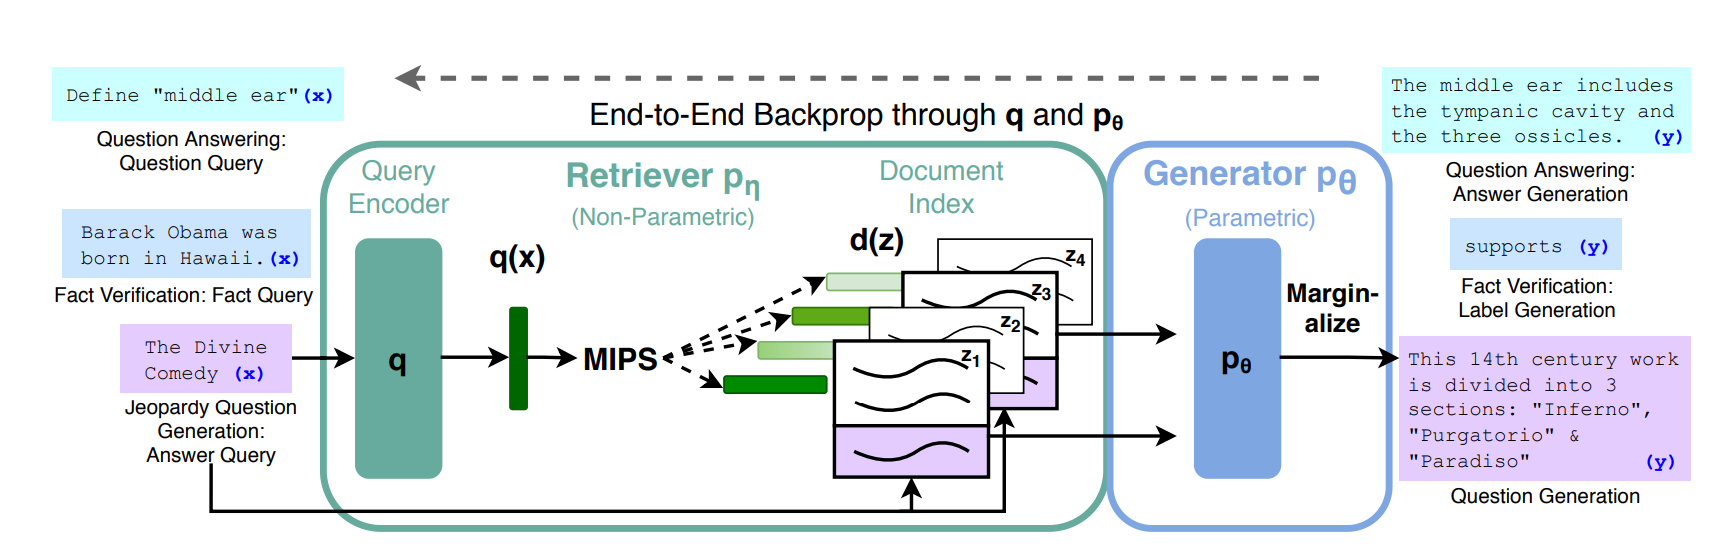
\includegraphics[width=\textwidth]{figuri/rag.png}
    \caption{Arhitectura modelului RAG \cite{lewis2020retrieval}}
    
\end{figure}

\subsection{Măsurarea similarității}

Atât interogarea utilizatorului, cât și fragmentele de text extrase din documente sunt transformate în reprezentări numerice, denumite embeddings. Acestea sunt reprezentate într-un spațiu vectorial, în care se evaluează gradul de similaritate semantică dintre interogare și fiecare fragment de text.

Similaritatea sau distanța dintre aceste reprezentări poate fi calculată utilizând diferite măsuri, alegerea acestora reprezentând un hiperparametru al sistemului. Cele mai utilizate metode includ similaritatea cosinus, produsul scalar sau distanța euclidiană.

\begin{figure}[H]
    \centering
    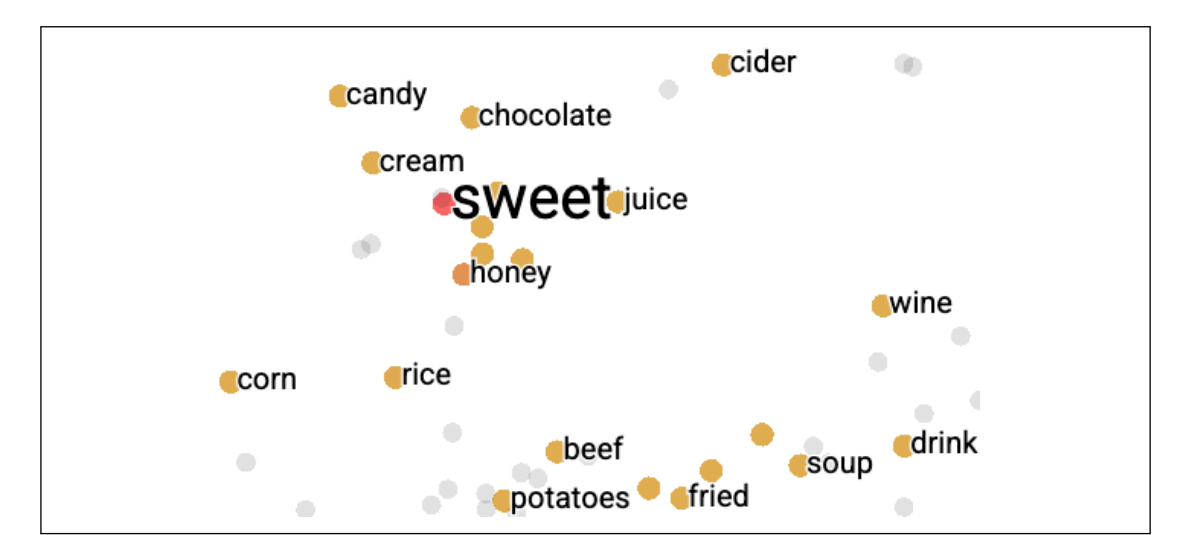
\includegraphics[width= 0.8\textwidth]{figuri/Distance.png}
    \caption{Vizualizarea în 2D a embedding-urilor Word2Vec, evidențiind gruparea semantică a cuvintelor similare (adaptat după \cite{mikolov2013word2vec})}
    
\end{figure}

\begin{itemize}
    \item\textbf{Similaritatea cosinus} este una dintre cele mai utilizate măsuri pentru compararea reprezentărilor vectoriale. Aceasta este definită ca raportul dintre produsul scalar al celor doi vectori și produsul normelor acestora:

\begin{equation}
\text{sim}_{cos}(P, Q) = \frac{P \cdot Q}{\|P\| \|Q\|}
\end{equation}

Din punct de vedere geometric, această măsură reprezintă cosinusul unghiului dintre cei doi vectori în spațiul vectorial. Valorile apropiate de 1 indică o similaritate semantică ridicată, în timp ce valorile apropiate de 0 sau negative indică o similaritate redusă. 

În unele cazuri, se utilizează și distanța cosinus, definită ca:

\begin{equation}
d_{cos}(P, Q) = 1 - \text{sim}_{cos}(P, Q)
\end{equation} 

    \item\textbf{Distanța euclidiană} reprezintă una dintre cele mai utilizate măsuri de distanță în spațiul vectorial, fiind aplicabilă în special pentru date numerice. Aceasta derivă din teorema lui Pitagora și cuantifică distanța directă dintre două puncte în spațiul vectorial.

\begin{equation}
d_{L_2}(P, Q) = \sqrt{\sum_{i=1}^{d} (P_i - Q_i)^2}
\end{equation}

Această măsură reflectă distanța geometrică dintre doi vectori, valori mai mici indicând o similaritate mai mare între aceștia.


\item\textbf{Distanța Manhattan}, cunoscută și sub denumirea de distanță L1 sau City Block Distance, reprezintă o măsură de distanță utilizată în spațiile vectoriale, în special pentru date numerice. Aceasta nu se bazează pe teorema lui Pitagora, ci pe suma diferențelor absolute dintre componentele vectorilor.

\begin{equation}
d_{L_1}(P, Q) = \sum_{i=1}^{d} |P_i - Q_i|
\end{equation}

Din punct de vedere geometric, această măsură reflectă distanța parcursă între două puncte atunci când deplasarea se face doar pe direcții ortogonale, similar deplasării într-o rețea urbană. Valorile mai mici indică o similaritate mai mare între vectori.

\item\textbf{Produsul scalar} reprezintă o măsură de similaritate între doi vectori, calculată ca suma produselor componentelor corespunzătoare:

\begin{equation}
P \cdot Q = \sum_{i=1}^{d} P_i Q_i
\end{equation}

Această măsură este utilizată frecvent în mecanismele de regăsire bazate pe embedding-uri, deoarece permite evaluarea rapidă a similarității dintre vectori. Totuși, spre deosebire de similaritatea cosinus, produsul scalar este influențat de magnitudinea vectorilor. \cite{levy2024similarity}
\end{itemize}
    \subsection{Avantaje și limitări ale RAG}
  

Modelele de tip Retrieval-Augmented Generation oferă o serie de avantaje semnificative față de modelele lingvistice clasice. Unul dintre principalele beneficii constă în capacitatea de a accesa informații externe în timpul generării, ceea ce permite îmbunătățirea acurateței răspunsurilor și reducerea riscului de generare a unor informații eronate. Prin utilizarea documentelor relevante ca sursă de context, modelele RAG pot produce răspunsuri mai bine fundamentate, în special în sarcinile care necesită cunoștințe detaliate sau actualizate.

Un alt avantaj important îl reprezintă separarea memoriei parametrice de cea non-parametrică, ceea ce permite actualizarea informațiilor fără a fi necesară reantrenarea completă a modelului. Astfel, sistemele bazate pe RAG pot integra rapid noi date prin actualizarea bazei de documente utilizate de componenta de regăsire.\cite{lewis2020retrieval}

Cu toate acestea, utilizarea arhitecturii RAG implică și o serie de limitări. Performanța modelului depinde în mod direct de calitatea mecanismului de regăsire, iar selectarea unor documente nerelevante poate conduce la generarea unor răspunsuri incorecte. În plus, integrarea componentei de regăsire introduce un cost computațional suplimentar și poate crește timpul de răspuns al sistemului. 


De asemenea, calitatea procesului de regăsire depinde în mod semnificativ de modul în care textul este fragmentat. O segmentare necorespunzătoare poate conduce la pierderea contextului semantic sau la extragerea unor informații incomplete, afectând relevanța documentelor recuperate. 

Prin urmare, eficiența modelelor de tip RAG depinde de echilibrul dintre calitatea mecanismului de regăsire și capacitatea modelului de generare de a integra informațiile selectate.

\section{Modele agentice și extinderea RAG}

În contextul sistemelor bazate pe Retrieval-Augmented Generation, integrarea unor mecanisme agentice permite extinderea fluxului clasic de procesare prin introducerea unor etape suplimentare de decizie și planificare. Astfel, modelul nu se limitează la regăsirea informației și generarea unui răspuns, ci poate selecta în mod dinamic sursele relevante, poate rafina interogările și poate adapta strategia de răspuns în funcție de obiectivul urmărit. 

Agentic AI descrie sisteme de inteligență artificială concepute pentru a lua decizii și a acționa în mod autonom, având capacitatea de a urmări obiective complexe cu un nivel redus de supraveghere. Aceste sisteme combină flexibilitatea modelelor lingvistice de mari dimensiuni (LLM) cu precizia abordărilor bazate pe programare tradițională.

Acest tip de inteligență artificială acționează autonom pentru atingerea unui obiectiv, utilizând tehnologii precum procesarea limbajului natural, învățarea automată, învățarea prin întărire și reprezentarea cunoștințelor. Spre deosebire de modelele generative clasice, care reacționează la intrarea utilizatorului, Agentic AI adoptă o abordare proactivă, fiind capabil să își adapteze comportamentul în funcție de context și de schimbările din mediul de execuție. \cite{ibm_agentic}

\begin{figure}[H]
    \centering
    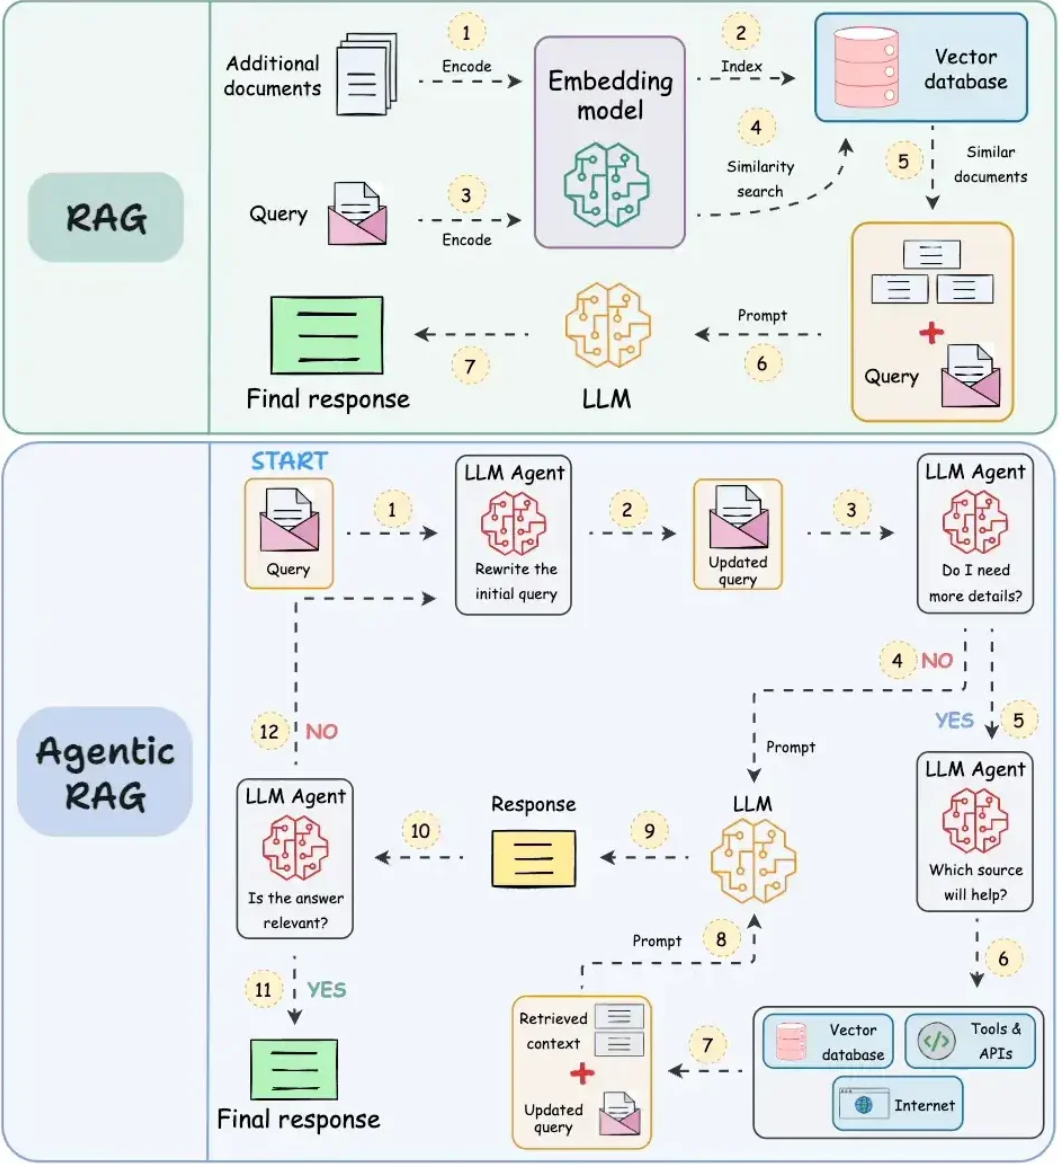
\includegraphics[width=0.8\textwidth]{figuri/agentic.png}
    \caption{Arhitectura unui sistem Agentic AI \cite{dextralabs}}
    
\end{figure}

\subsection{Generative AI vs Agentic AI}

Pentru a evidenția diferențele dintre principalele tipuri de sisteme de inteligență artificială, se poate realiza următoarea clasificare conceptuală. Sistemele tradiționale de inteligență artificială sunt orientate către furnizarea unui răspuns la o întrebare specifică. Modelele de tip generativ (Generative AI) au capacitatea de a crea conținut nou pe baza datelor de antrenare. În cazul agenților AI, aceștia execută sarcini specifice pe baza unor reguli sau instrucțiuni predefinite.

În schimb, sistemele de tip Agentic AI se disting printr-un grad mai ridicat de autonomie, fiind capabile să stabilească obiective, să elaboreze planuri pentru atingerea acestora, să execute acțiuni și să își adapteze comportamentul pe baza rezultatelor obținute. \cite{agentic_medium}



\cleardoublepage
\chapter{Prezentarea tehnologiilor folosite}
\section{Limbajul de programare și organizarea aplicației}
Implementarea aplicației este realizată în Python 3.10, limbaj ales datorită ecosistemului matur pentru procesarea limbajului natural, integrarea modelelor lingvistice și dezvoltarea rapidă a prototipurilor. Arhitectura software este organizată modular, cu separarea clară a responsabilităților între orchestrare, mecanisme de protecție, evaluare, regăsire contextuală, ingestie și interfața API. Această structură facilitează atât testarea independentă a componentelor, cât și extinderea ulterioară a sistemului.

\section{Interfața API}
Pentru expunerea funcționalităților aplicației este utilizat framework-ul Flask. Interfața API oferă endpoint-uri dedicate fluxului intern, dar și endpoint-uri compatibile cu formatul OpenAI Chat Completions, ceea ce permite integrarea directă cu OpenWebUI. Această compatibilitate asigură interoperabilitatea cu instrumente existente și reduce efortul necesar pentru integrarea într-un flux de utilizare conversațională.

\section{Tehnologiile RAG: vectori, chunking și căutare semantică}
Componenta Retrieval-Augmented Generation utilizează Qdrant ca bază de date vectorială pentru stocarea embedding-urilor și regăsirea fragmentelor relevante. În fluxul curent, embedding-urile sunt generate prin clientul OpenAI, iar documentele sunt indexate împreună cu metadate necesare pentru trasabilitate și citare.

Segmentarea documentelor este realizată prin două strategii complementare. Prima strategie este una euristică, bazată pe structurarea textului în secțiuni și paragrafe. A doua strategie utilizează chunking semantic prin LlamaIndex (\texttt{llama-index-core}), cu scopul de a obține fragmente mai coerente din punct de vedere contextual. În cazul în care dependențele necesare pentru chunking semantic nu sunt disponibile, sistemul revine controlat la metoda euristică, menținând stabilitatea procesului de ingestie.

\section{Modele lingvistice și rutare multi-provider}
Sistemul este proiectat pentru a opera cu mai mulți furnizori LLM, integrați printr-un strat comun de rutare. În implementarea actuală sunt folosiți furnizori cloud, precum OpenAI și Anthropic, dar și furnizori locali prin Ollama (de exemplu, modele Gemma sau Qwen). Această abordare permite mecanisme de fallback în scenariile în care evaluarea răspunsului nu este satisfăcătoare sau unul dintre furnizori devine indisponibil. În consecință, aplicația poate funcționa atât în configurații bazate pe servicii externe, cât și în configurații locale.

\section{Componenta de graf de cunoștințe}
Pentru extinderea capabilităților de regăsire, proiectul include o componentă Graph-RAG bazată pe Kuzu. Aceasta permite reprezentarea explicită a entităților și relațiilor extrase din documente, completând regăsirea vectorială clasică. În scenariile hibride, contextul este construit prin combinarea rezultatelor vectoriale cu informațiile obținute din graf, ceea ce poate crește relevanța răspunsului în întrebările cu dependențe semantice mai complexe.

\section{Procesarea datelor și utilitare}
Etapa de ingestie se bazează pe mai multe biblioteci specializate. PyMuPDF este utilizat pentru extracția textului din fișiere PDF, iar pandas pentru prelucrarea datelor din surse tabelare, precum CSV sau JSON. Configurarea aplicației este gestionată prin python-dotenv, care permite controlul parametrilor de execuție prin variabile de mediu. Pentru apeluri HTTP auxiliare în fluxurile de date este utilizată biblioteca httpx.

\section{Containerizare și rulare}
Pentru asigurarea reproductibilității mediului de execuție și a unei instalări rapide, aplicația este containerizată cu Docker. Orchestrarea serviciilor este realizată cu Docker Compose, într-o topologie care include aplicația principală, serviciul API, Qdrant, OpenWebUI și, opțional, Ollama pentru inferență locală. Această organizare permite rularea consecventă a sistemului atât în mediul de dezvoltare, cât și în scenarii de demonstrare.

\section{Calitatea codului și testare}
Controlul calității codului este susținut prin instrumente de analiză statică și testare automată. Black și Ruff sunt utilizate pentru formatare și verificări de stil, iar coverage este folosit pentru monitorizarea acoperirii testelor. În plus, proiectul include o suită de teste orientată către componentele critice, precum guardrails, orchestrare, retrieval și ingestie, cu scopul de a menține stabilitatea funcțională pe măsură ce aplicația evoluează.

\chapter{Arhitectura proiectului}
\section{Fluxul operațional al agentului principal}

Arhitectura implementată în cadrul proiectului urmează un flux secvențial de procesare, proiectat pentru a reduce riscul de răspunsuri incorecte în context medical:
\begin{enumerate}
    \item aplicarea mecanismelor de protecție (\textit{guardrails}) asupra întrebării utilizatorului;
    \item decizia dacă este necesară recuperarea de context din baza vectorială (RAG);
    \item extragerea fragmentelor relevante atunci când interogarea necesită cunoștințe externe;
    \item construirea promptului final prin combinarea regulilor din fișierul \texttt{llm.txt}, a contextului recuperat și a întrebării utilizatorului;
    \item trimiterea promptului către LLM Hub și generarea răspunsului;
    \item evaluarea răspunsului cu un evaluator dedicat;
    \item reluarea procesului, cu prompt ajustat sau cu schimbarea furnizorului LLM, dacă evaluarea nu este satisfăcătoare;
    \item returnarea către utilizator doar a răspunsului validat.
\end{enumerate}

\section{Componentele sistemului}
Sistemul este organizat modular, astfel încât fiecare etapă critică să poată fi testată și îmbunătățită independent:
\begin{itemize}
    \item modulul de protecție (\textit{guardrails}) pentru filtrarea interogărilor și gestionarea cerințelor sensibile;
    \item modulul de regăsire contextuală (bază vectorială + indexare semantică);
    \item orchestratorul agentic pentru decizie, construcție de prompt și selecția furnizorului LLM;
    \item evaluatorul de răspuns pentru validare automată și controlul calității.
\end{itemize}

\chapter{Interpretarea rezultatelor}
\section{Metodologie de evaluare}
Evaluarea urmărește atât calitatea factuală a răspunsului, cât și conformitatea cu regulile de siguranță. Pentru fiecare întrebare din setul de test se analizează relevanța contextului recuperat, coerența răspunsului generat și verdictul evaluatorului automat.

\section{Analiză comparativă}
Rezultatele sunt comparate între modele și furnizori pe baza unor criterii comune: acuratețe, consistență, timp de răspuns și rată de validare la prima încercare. În plus, se evidențiază cazurile în care mecanismul de reluare a îmbunătățit rezultatul final.

\chapter{Concluzii}
\section{Concluzii generale}
Lucrarea evidențiază faptul că integrarea LLM cu RAG și cu un flux agentic de validare poate crește fiabilitatea răspunsurilor în domeniul medical, cu condiția utilizării unor surse bine curate și a unor mecanisme explicite de control al calității.

\section{Direcții viitoare}
Extinderile naturale includ optimizarea strategiei de recuperare a contextului, îmbunătățirea evaluatorului prin criterii mai fine și integrarea unui mecanism de citare automată a surselor în răspunsul final.

\bibliographystyle{unsrt}
\bibliography{referinte}


\appendix
\chapter{Exemplu de prompt utilizat în orchestrare}
\begin{verbatim}
Rol: asistent medical educațional, orientat pe informație verificabilă.
Instrucțiuni:
- folosește exclusiv contextul furnizat și reguli din llm.txt;
- când contextul este insuficient, declară limitarea explicit;
- nu oferi diagnostic final și nu înlocui consultația medicală.

Context RAG:
{chunk_1}
{chunk_2}
...

Întrebarea utilizatorului:
{user_query}
\end{verbatim}





\end{document}
